\chapter{Fonctions}

\section{Généralités}

Les fonctions jouent un rôle important dans toute organisation. Par exemple, la fonction "élève" donne certains droits et certains devoirs à une personne. 
Les feux de circulation donnent un autre type de fonction : le vert signifie qu'on peut avancer et le rouge qu'on doit s'arrêter.

Il existe beaucoup d'autres exemples. Celui que nous retiendrons car il est le plus en lien avec la notion mathématique de fonction se trouve dans tous les magasins. La caisse enregistreuse attribue à chaque objet un prix selon sa nature et son poids. Il serait ennuyeux qu'un article ait plusieurs prix ou qu'il manque le prix d'un article. Par contre si rien dans le magasin ne coûte 5 frs, il n'y a pas de problème.

\begin{definition}\index{fonction}
Une \emph{fonction} est une association entre deux ensembles $A$ et $B$ telle que tout élément de l'ensemble $A$, appelé \emph{ensemble de départ}, est associé à exactement un élément de l'ensemble $B$, appelé \emph{ensemble d'arrivée}.

Les éléments de l'ensemble de départ sont appelés les \emph{préimages} et ceux de l'ensemble d'arrivée les \emph{images}.
\end{definition}

Une fonction est représentable par bien des façons (cahier des charges, code barre, etc). En mathématiques on utilisera tout d'abord des flèches.

\begin{exemple}
La fonction suivante décrit les liens entre l'ensemble $A=\{ a,b,c,d\}$ et ${B=\{ 1,2,3\}}$ :
$$
\xymatrix@1{
a \ar[rrrdd] &&& 1 \\
b \ar[rrru] &&& 2 \\
c \ar[rrr] &&& 3 \\
d \ar[rrruu] &&& 4
}
$$
  
On voit que les objets $a$ et $c$ sont associés à $3$ et que rien n'est associé à $4$. Cela ne cause pas de problème, car si l'on revient à l'exemple des prix, cela signifie que $a$ et $c$ ont le même prix et que rien de coûte $2$.

Par contre, l'association ci-dessous n'est pas une fonction :
$$
\xymatrix@1{
a \ar[rrrdd] \ar[rrrddd] &&& 1 \\
b \ar[rrru] &&& 2 \\
c \ar[rrr] &&& 3 \\
d &&& 4
}
$$
car $a$ est associé à deux nombres, $1$ et $4$ et $d$ à aucun nombre.
\end{exemple}

\section{Fonction numérique}

Lorsque l'ensemble de départ et d'arrivée sont des sous-ensemble de $\R$, on parle de \emph{fonction numérique}.\index{fonction!numérique}

La plupart des fonctions numériques que nous allons voir ne sont pas aléatoires; c'est-à-dire qu'il y a une règle pour associer deux éléments. Nous allons utiliser la lettre $x$ pour savoir ce qui se passe pour l'élément de l'ensemble de départ.

\begin{exemple}
\'Etudions de plus près la fonction $f(x) = 2x+1$ : elle signifie que l'élément de départ est multiplié par $2$, puis qu'on ajoute $1$ au résultat. Ainsi
$$
\begin{array}{rcl}
3 &\longrightarrow & (2\cdot 3) + 1 = 7\\
-5 &\longrightarrow &  (2 \cdot (-5))+1 = -9 \\
\dots & & \\
\end{array}
$$
On peut aussi représenter cette fonction à l'aide d'un tableau :
$$
\begin{array}{|l|l|l|l|l|l|}
\hline
x & -2 & -1 & 0 & 1 & 2\\
\hline
f(x) & -3 & -1 & 1 & 3 & 5 \\
\hline
\end{array}
$$
ou par un ensemble de couples :
$$
f(x) = \{\dots, (-2;-3), (-1;-1), (0;1), (1,3), (2,5), \dots \}
$$
Pour l'instant, nous n'avons utilisé que des nombres entiers dans l'ensemble de départ, mais les nombres fractionnaires conviennent aussi bien :
$$
f(\frac{3}{5}) = 2\cdot \frac{3}{5} + 1 = \frac{6}{5} + \frac{5}{5} = \frac{11}{5}
$$
ainsi que toutes les autres sortes de nombres. L'ensemble des paires d'une fonction contient donc un nombre infini d'éléments. Il serait assez intéressant de pouvoir représenter cet ensemble autrement que par une liste de paires.

Or, justement, il existe une manière de représenter une paire sur une feuille :

\subsection{Représentation}\label{fct_representation}
 
\begin{enumerate}
\item on commence par dessiner deux droites perpendiculaires, graduées de manière à ce que le zéro soit sur le point d'intersection.
\item on place le point ainsi : en horizontal on se déplace du premier nombre de la paire et en vertical du second.
\end{enumerate}
\begin{center}
\includegraphics{affines/fct_intro.png}
\end{center}
\end{exemple}

\begin{definition}\index{fonction!graphe}
Le \emph{graphe d'une fonction} est la représentation de toutes les paires d'une fonction. En écriture mathématique, on note :
$$
\mathcal{C}_f = \{(x;f(x))\in \R^2 \; | \; x\in D_f\}
$$
où $D_f$ est l'ensemble de départ de la fonction $f$.
\end{definition}

\begin{exemple}
La représentation de la fonction $f(x) = 2x+1$ est donnée par
\begin{center}
\includegraphics{affines/fct_intro_graphe.png}
\end{center}
Nous verrons par la suite comment représenter le graphe de ce type de fonction.
\end{exemple}

\begin{definition}\index{fonction!continue}
Une fonction est dite \emph{continue} si son graphe peut être représenté sans lever le crayon.
\end{definition}

La "vraie" définition est de fait plus complexe, mais celle-ci nous conviendra.

De fait, pour les fonctions continues (et aussi pour la plupart des autres), le graphe suffit à tout connaître de la fonction.

\begin{exemple}
Le graphe de la fonction est le suivant :
\begin{center}
\includegraphics{affines/fct_graphe.png}
\end{center}
on cherche à connaître l'image de $2$ (c'est-à-dire le nombre associé à $2$). On regarde alors où la verticale de $2$ coupe le graphe et surtout à quelle hauteur elle le fait :
\begin{center}
\includegraphics{affines/fct_graphe_sol.png}
\end{center}
Ainsi l'image de $2$ est $-4$.
\end{exemple}

Quelques croisements particuliers sont plus intéressants :
\begin{definition}
Le ou les \emph{zéros de fonction}\index{fonction!zéro} sont les intersections du graphe de la fonction avec l'axe horizontal. On peut les calculer en résolvant l'équation
$$
f(x) = 0.
$$
L'\emph{ordonnée à l'origine}\index{fonction!ordonnée à l'origine} est l'intersection du graphe avec l'axe vertical. On peut la calculer en cherchant l'image de zéro :
$$
f(0) = ?
$$
\end{definition}

\subsection{Signes}

\'Etudier les signes d'une fonction numérique\index{fonction!signes} revient à donner l'ensemble des valeurs qui sont envoyées sur un nombre positif et réciproquement l'ensemble des valeurs qui sont envoyées sur un nombre négatif.

Or le nombre sur lequel est envoyé une valeur représente la coordonnée verticale. Ainsi les valeurs qui sont envoyées sur un nombre positif seront représentée au-dessus de l'abscisse et celles sur un nombre négatif en-dessous.

\begin{exemple}
Pour la fonction $f(x) = 3x^2 -4x -1$, le nombre $2$ fait partie des valeurs qui sont envoyées sur un nombre positif, car $3\cdot 2^2 - 4\cdot 2 - 1 = 3 >0$, alors que le nombre $1$ fait partie des valeurs qui sont envoyées sur un nombre négatif car $3\cdot 1^2 - 4 \cdot 1 -1 = -2 <0$.
\end{exemple}

\begin{definition}
On dit que $f$ est de \emph{signe positif} sur un ensemble de valeur si chacun des éléments de l'ensemble est envoyé par $f$ sur un nombre positif.

On dit que $f$ est de \emph{signe négatif} sur un ensemble de valeur si chacun des éléments de l'ensemble est envoyé par $f$ sur un nombre négatif.
\end{definition}

Graphiquement, une fonction est de signe positif si son graphe est au-dessus de l'abscisse et de signe négatif s'il est au-dessous.

\begin{exemple}
Sur le graphe ci-dessous :
\begin{center}
\includegraphics[scale=0.4]{affines/fct_signe.png}
\end{center}
La fonction $f$ est positive quand $x$ est plus petit que $-3$ ou quand $x$ est plus grand que $2$. La fonction $f$ est négative quand $x$ est compris entre $-3$ et $2$. En effet
\begin{center}
\includegraphics{affines/fct_signe_ex.png}
\end{center}

On le note :
$$
\begin{array}{|c|c|c|c|c|c|c|c|}
\hline
x & -\infty & & -3 & & 2 & & +\infty \\
\hline
f(x) & + & + & 0 & - & 0 & + & + \\
\hline
\end{array}
$$
\end{exemple}

\begin{theoreme}
Soit $f$ une fonction continue. Alors le signe de la fonction $f$ ne peut changer que sur un zéro de fonction.
\end{theoreme}

\begin{proof}
En effet, on ne peut passer d'un côté et de l'autre de l'abscisse sans lever le crayon qu'en la coupant. Or c'est la définition d'un zéro de fonction.
\end{proof}

\subsection{Variation}

Bien que la variation ait une définition analytique, nous n'en verrons que la définition géométrique :

\begin{definition}
Une fonction a une variation positive si son graphe "monte" et négative si son graphe "descend".
\end{definition}

\begin{exemple}
La fonction ayant le graphe suivant :
\begin{center}
\includegraphics{affines/fct_var.png}
\end{center}
Monte jusqu'à $(-1,79;8,21)$, descend jusqu'à $(1,12;-4,06)$ puis monte. On peut donner le tableau de variation suivant :
$$
\begin{array}{|c|c|c|c|c|c|c|c|}
x& -\infty & & -1,79 & & 1,12 & & +\infty \\
\hline
f(x) & \nearrow & \nearrow & 8,81 & \searrow & -4,06 & \nearrow & \nearrow \\
\end{array}
$$
\end{exemple}

\begin{definition}
On appelle \emph{extremum}\index{fonction!extremum} le point où une fonction change de variation. 

Si le graphe fait une "bosse", il s'agit d'un \emph{maximum}\index{fonction!maximum} et s'il fait un "creux", d'un \emph{minimum}\index{fonction!minimum}.
\end{definition}

\section{Fonction affine} \label{fct_affine}

Intéressons-nous maintenant à un type bien particulier de fonction : les fonctions affines\index{fonction!affine}. Ces derniers sont du type 
$$
f(x) = ax + b
$$
où $a$ et $b$ sont des nombres réels. Par exemple la fonction $f(x) = 2x + 3$ est une fonction affine ($a=2$ et $b=3$), la fonction $f(x) = 4-x$ aussi ($a=-1$ et $b=4$), mais la fonction $f(x) = 3x^2 + 2$ n'en est pas une.

\subsection{Représentation}

Le graphe d'une fonction affine est donné par une droite.

\begin{exemple}
Le graphe suivant représente la fonction $f(x) = 2x+3$ :
\begin{center}
\includegraphics{affines/fct_affine.png}
\end{center}
\end{exemple}

Ainsi pour représenter une fonction affine, il suffit de trouver deux points sur le plan qui appartiennent au graphe de la fonction. Or nous avons déjà parlé de deux points particuliers qui représentent l'intersection du graphe et des axes : le zéro de fonction\index{fonction!zéro} et l'ordonnée à l'origine\index{fonction!ordonnée à l'origine}. Il suffit donc de trouver ces deux points pour pouvoir représenter une fonction affine.

\begin{exemple}
Représenter le graphe de la fonction affine
$$
f(x) = 2x-4.
$$
Commençons par trouver le zéro de $f$ : il s'agit de trouver quelle(s) valeur(s) de $x$ sont envoyés sur $0$ par $f$, c'est-à-dire de résoudre l'équation
$$
\begin{array}{lcl}
2x-4 &=& 0 \ssi\\
2x &=& 4 \ssi \\
x &=& 2.
\end{array}
$$
Ainsi le premier point est donné par le zéro de fonction $(2;0)$, car $2$ est envoyé sur $0$ par le fonction $f$.

Ensuite, il s'agit de trouver sur quelle valeur est envoyé $0$. On fait simplement le calcul :
$$
f(0) = 2\cdot 0 -4 = 0-4 = -4.
$$
Le deuxième point est donné par l'ordonnée à l'origine $(0;-4)$, car $0$ est envoyé sur $-4$ par la fonction $f$.

On obtient donc le graphe suivant :
\begin{center}
\includegraphics{affines/fct_affine_ex.png}
\end{center}
\end{exemple}

\subsection{Pente}

Puisqu'une fonction affine est représentée par une droite, on peut lui associer la notion de \emph{pente}\index{pente!d'une fonction affine}.

\begin{definition}\label{pente1}
Pour une droite, la \emph{pente} est donnée par la formule :
$$
\mbox{pente} = \frac{\mbox{dénivellation}}{\mbox{distance horizontale}}
$$
\end{definition}

\begin{theoreme}\label{thm:pente}
La pente de la fonction affine
$$
f(x) = ax + b
$$
est donnée par $a$.
\end{theoreme}

\begin{proof}
En effet, prenons $x_1$ et $x_2$ deux nombres réels. Alors le graphe de la fonction affine passe par les points $\left(x_1;f(x_1)\right)$ et $\left(x_2 ; f(x_2) \right)$.
\begin{center}
\includegraphics{affines/fct_pente.png}
\end{center}
Selon la définition :
$$
\begin{array}{lcl}
\mbox{pente} &=& \frac{f(x_2)-f(x_1)}{(x_2-x_1)} \\
&=& \frac{(ax_2+b)-(ax_1+b)}{(x_2-x_1}\\
&=& \frac{ax_2+b-ax_1-b}{(x_2-x_1}\\
&=& \frac{ax_2-ax_1}{(x_2-x_1}\\
&=& \frac{a(x_2-x_1)}{(x_2-x_1}\\
&=& a \\
\end{array}
$$
ce qui démontre le théorème.
\end{proof}

Puisque la pente représente la différence de hauteur lorsque l'on va de gauche à droite en suivant le graphe, 
$$
\left\{
\begin{array}{lcl}
\mbox{Si } a>0 &\mbox{ alors} &\mbox{ la droite "monte"}\\
\mbox{Si } a<0 &\mbox{ alors} &\mbox{ la droite "descend"}\\
\mbox{Si } a=0 &\mbox{ alors} &\mbox{ la droite est "plate"}\\
\end{array}
\right.
$$


\subsection{Signes et variations}

Grâce au théorème~\ref{thm:pente}, on peut immédiatement poser le raisonnement suivant :

Si $a$ est positif, la droite monte et donc part des négatifs pour aller aux positifs. A contrario, si $a$ est négatif, la droite descend et donc part des positifs pour aller aux négatifs. On peut résumer ça ainsi :

$$
\left\{
\begin{array}{lcll}
\mbox{Si } a>0 &\mbox{ alors} &\mbox{variation = } \nearrow \mbox{ et }& \mbox{signes :} - 0 +\\
\mbox{Si } a<0 &\mbox{ alors} &\mbox{variation = } \searrow \mbox{ et }& \mbox{signes :} + 0 -\\
\mbox{Si } a=0 &\mbox{ alors} &\mbox{variation = } \rightarrow \mbox{ et }& \mbox{signes constant }\\
\end{array}
\right.
$$

\subsection{Cas particuliers}

\begin{definition}
Les fonctions affines ayant $a=0$ sont appelées des fonctions \emph{constantes}\index{fonction!constante} et celles ayant $b=0$, fonctions \emph{linéaires}\index{fonction!linéaire}.
\end{definition}

\begin{proposition}
Une fonction affine est constante si et seulement si elle a un graphe "plat" et une fonction affine est linéaire si et seulement si elle passe par $(0;0)$.
\end{proposition}

\begin{proof}
Avec ce que nous avons vu auparavant, il est assez facile de démontrer qu'une fonction constante à un graphe plat. En effet, si c'est une fonction constante, alors $a=0$ est donc son graphe ne monte ni ne descend; il est plat. Avec la même facilité, une fonction linéaire passe par $(0;0)$. En effet, si $f$ est une fonction linéaire, alors $f(0) = a\cdot 0 + 0 = 0$ et donc son graphe passe par le point $(0;0)$.

L'inverse est un peu plus compliqué.

Soit $f$ une fonction affine ayant un graphe "plat". Alors sa pente ne peut pas être supérieure à $0$, car elle monterait, ni inférieure à $0$, car elle descendrait. Ainsi $f$ a une pente égale à zéro, c'est-à-dire $a=0$. Ainsi $f$ est bien une fonction constante.

Montrons maintenant qu'une fonction affine passant par $(0;0)$ est une fonction linéaire. Soit donc la fonction $f(x) = ax +b$ dont le graphe passe par $(0;0)$. Cela revient à dire que l'image de $0$ par $f$ est aussi $0$ :
$$
\begin{array}{lcl}
f(0) &=& 0 \ssi\\
a\cdot 0 + b &=& 0 \ssi\\
b &=& 0
\end{array}
$$
Ainsi, puisque $b=0$, la fonction affine $f$ est une fonction linéaire, ce qui termine la démonstration du théorème.
\end{proof}

\section{\'Etude de fonction affine}\index{Etude de fonction!affine}\label{affine}

Historiquement, les études de fonctions servaient à représenter au mieux leur graphe à une époque où les ordinateurs n'existaient pas. Actuellement, grâce à la puissance de l'informatique, toute fonction peut être représentée à l'aide de l'informatique. Par exemple, pour représenter une fonction $f$ quelconque pour des valeurs de $x$ comprises entre $0$ et $1$1, il suffit de calculer les images de $f$ entre $0$ et $1$ en prenant un écart de $0.001$. Cent calculs seront nécessaires, ce qui ne prend qu'une fraction de seconde à un ordinateur, mais bien plus à un être humain normalement constitué.

Les études de fonctions que nous verrons n'auront donc pas pour finalité la représentation du graphe, mais plutôt la mobilisation de l'ensemble des savoirs inhérents au type de fonction étudiée.

Une étude de fonction affine passera par les points suivants :
\begin{enumerate}
\item Pente
\item Zéro de $f$
\item Ordonnée à l'origine de $f$
\item Tableau des signes et des variations
\item Représentation du graphe
\end{enumerate}

\begin{exemple}
\'Etude de la fonction 
$$
f(x) = 3x+1
$$
\begin{enumerate}
\item Pente : $a=3$
\item Zéro $f(x) = 0 \ssi 3x+1 = 0 \ssi 3x = -1 \ssi x = \frac{-1}{3}$
\item Ordonnée à l'origine : $f(0) = 3\cdot0 + 1 = 1$
\item Signe et variation
$$
\begin{array}{c|ccccc}
x & -\infty & & \frac{-1}{3} & & +\infty\\
\hline
f(x) &-& - & 0 & + & +\\
\hline
\mbox{var} &\nearrow & \nearrow & & \nearrow & \nearrow\\
\end{array}
$$
\item Graphe
\begin{center}
\includegraphics[width=0.5\textwidth]{affines/ensemble.png}
\end{center}
\end{enumerate}
\end{exemple}
\section{Exercices}
\begin{exercice}
Étudier complètement les fonctions suivantes.
	Tracer au maximum deux droites sur un même système d'axes, unité des axes : un carré.
\begin{multicols}{3}
\begin{enumerate}
\item $f(x)=x+1$
\item $f(x)=x-3$
\item $f(x)=2x-3$
\item $f(x)=2x+5$ 
\item $f(x)=\frac{x}{2}+1$ 
\item $f(x)=-x+1$
\item $f(x)=-x-3$
\item $f(x)=-2x-3$
\item $f(x)=5x+8$
\item $f(x)=\frac{2x}{5}-3$
\item $f(x)=5x-5$
\item $f(x)=-10x+3$
\item $f(x)=-3x+7$
\item $f(x)=\frac{3x}{8}-2$
\item $f(x)=-\frac{x}{8}-1$
\item $f(x)=5$
\item $f(x)=-4$
\item $f(x)=3x$
\item $f(x)=-6x$
\item $f(x)=\frac{5x}{7}$
\end{enumerate}
\end{multicols}
\end{exercice}

\section{Corrigés}
\begin{solution}
$f(x)=x+1$
\begin{itemize}
\item Pente :	 
\item Ordonnée à l’origine :	$x=0\Rightarrow f(x)=1$ 
\item Zéro de fonction :	$f(x)=0\Rightarrow x=-1$
\item Signe et variation :	
$$\begin{array}{l|l|l|l|l|l}
x    & -\infty &   & -1 &   & +\infty \\
\hline
f(x) & -       & - & 0  & + & +   \\
 & -\infty & \nearrow & \nearrow & \nearrow & +\infty \\   
\end{array}$$
\item Graphique
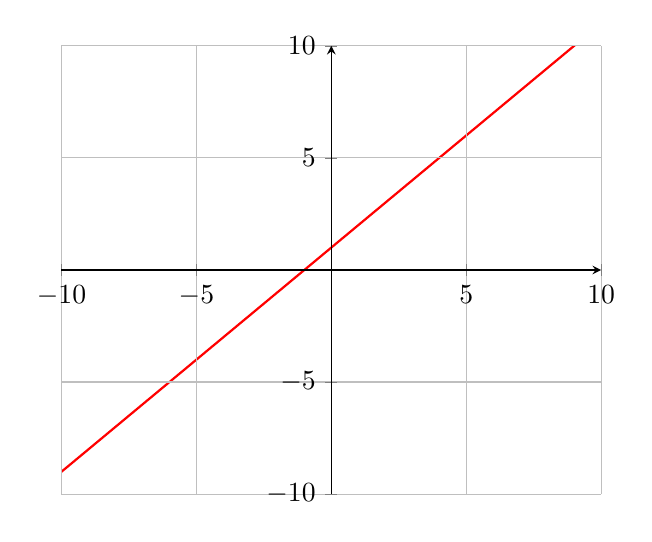
\begin{tikzpicture}
\begin{axis}[
	grid= major,
    xmin=-10, xmax=10,
    ymin=-10, ymax=10,
    axis lines=center,
    axis on top=true,
    domain=-10:10,
    ]

    \addplot [mark=none,draw=red, thick] {x+1};
\end{axis}
\end{tikzpicture}
\end{itemize}
\end{solution}

\begin{solution}
$f(x)=x-3$
\begin{itemize}
\item Pente :	$a=1$
\item Ordonnée à l’origine :	$x=0\Rightarrow f(x)=-3$
\item Zéro de fonction :	$f(x)=0\Rightarrow x=3$
\item Signe :	
$$\begin{array}{l|l|l|l|l|l}
x    & -\infty &   & 3 &   & +\infty \\
\hline
f(x) & -       & - & 0  & + & +      \\
& -\infty & \nearrow & \nearrow & \nearrow & +\infty \\   
\end{array}$$
\item Graphique
\begin{tikzpicture}
\begin{axis}[
    xmin=-10, xmax=10,
    ymin=-10, ymax=10,
    axis lines=center,
    axis on top=true,
    domain=-10:10,
    ]

    \addplot [mark=none,draw=red, thick] {x-3};
\end{axis}
\end{tikzpicture}
\end{itemize}
\end{solution}

\begin{solution}
$f(x)=2x-3$
\begin{itemize}
\item Pente :	$a=2$
\item Ordonnée à l’origine :	$x=0\Rightarrow f(x)=-3$
\item Zéro de fonction :	$f(x)=0\Rightarrow x=\frac{3}{2}$
\item Signe :	
$$\begin{array}{l|l|l|l|l|l}
x    & -\infty &   & \frac{3}{2} &   & +\infty \\
\hline
f(x) & -       & - & 0  & + & +      
\end{array}$$
\item Graphique
\begin{tikzpicture}
\begin{axis}[
    xmin=-10, xmax=10,
    ymin=-10, ymax=10,
    axis lines=center,
    axis on top=true,
    domain=-10:10,
    ]

    \addplot [mark=none,draw=red, thick] {2*x-3};
\end{axis}
\end{tikzpicture}
\end{itemize}
\end{solution}

\begin{solution}
$f(x)=2x+5$
\begin{itemize}
\item Pente :	$a=2$
\item Ordonnée à l’origine :	$x=0\Rightarrow f(x)=5$
\item Zéro de fonction :	$f(x)=0\Rightarrow x=-\frac{5}{2}$
\item Signe :	
$$\begin{array}{l|l|l|l|l|l}
x    & -\infty &   & -\frac{5}{2} &   & +\infty \\
\hline
f(x) & -       & - & 0  & + & +   \\
 & -\infty & \nearrow & \nearrow & \nearrow & +\infty \\   
\end{array}$$
\item Graphique
\begin{tikzpicture}
\begin{axis}[
    xmin=-10, xmax=10,
    ymin=-10, ymax=10,
    axis lines=center,
    axis on top=true,
    domain=-10:10,
    ]

    \addplot [mark=none,draw=red, thick] {2*x+5};
\end{axis}
\end{tikzpicture}
\end{itemize}
\end{solution}

\begin{solution}
$f(x)=\frac{x}{2}+1$
\begin{itemize}
\item Pente :	$a=\frac{1}{2}$
\item Ordonnée à l’origine :	$x=0\Rightarrow f(x)=1$
\item Zéro de fonction :	$f(x)=0\Rightarrow x=-2$
\item Signe :	
$$\begin{array}{l|l|l|l|l|l}
x    & -\infty &   & -2 &   & +\infty \\
\hline
f(x) & -       & - & 0  & + & +   \\
 & -\infty & \nearrow & \nearrow & \nearrow & +\infty \\   
\end{array}$$
\item Graphique
\begin{tikzpicture}
\begin{axis}[
    xmin=-10, xmax=10,
    ymin=-10, ymax=10,
    axis lines=center,
    axis on top=true,
    domain=-10:10,
    ]

    \addplot [mark=none,draw=red, thick] {x/2+1};
\end{axis}
\end{tikzpicture}
\end{itemize}
\end{solution}

\begin{solution}
$f(x)=-x+1$
\begin{itemize}
\item Pente :	$a=-1$
\item Ordonnée à l’origine :	$x=0\Rightarrow f(x)=1$
\item Zéro de fonction :	$f(x)=0\Rightarrow x=1$
\item Signe :
$$\begin{array}{l|l|l|l|l|l}
x    & -\infty &   & 1 &   & +\infty \\
\hline
f(x) & +       & + & 0  & - & -   \\
 & +\infty & \searrow & \searrow & \searrow & -\infty \\   
\end{array}$$
\item Graphique
\begin{tikzpicture}
\begin{axis}[
    xmin=-10, xmax=10,
    ymin=-10, ymax=10,
    axis lines=center,
    axis on top=true,
    domain=-10:10,
    ]

    \addplot [mark=none,draw=red, thick] {-x+1};
\end{axis}
\end{tikzpicture}
\end{itemize}
\end{solution}

\begin{solution}
$f(x)=-x-3$
\begin{itemize}
\item Pente :	$a=-1$
\item Ordonnée à l’origine :	$x=0\Rightarrow f(x)=-3$
\item Zéro de fonction :	$f(x)=0\Rightarrow x=-3$
\item Signe :	
$$\begin{array}{l|l|l|l|l|l}
x    & -\infty &   & -3 &   & +\infty \\
\hline
f(x) & +       & + & 0  & - & -   \\
 & +\infty & \searrow & \searrow & \searrow & -\infty \\   
\end{array}$$
\item Graphique
\begin{tikzpicture}
\begin{axis}[
    xmin=-10, xmax=10,
    ymin=-10, ymax=10,
    axis lines=center,
    axis on top=true,
    domain=-10:10,
    ]

    \addplot [mark=none,draw=red, thick] {-x-3};
\end{axis}
\end{tikzpicture}
\end{itemize}
\end{solution}

\begin{solution}
$f(x)=-2x-3$
\begin{itemize}
\item Pente :	$a=-2$
\item Ordonnée à l’origine :	$x=0\Rightarrow f(x)=-3$
\item Zéro de fonction :	$f(x)=0\Rightarrow x=-\frac{3}{2}$
\item Signe :	
$$\begin{array}{l|l|l|l|l|l}
x    & -\infty &   & -\frac{3}{2} &   & +\infty \\
\hline
f(x) & +       & + & 0  & - & -   \\
 & +\infty & \searrow & \searrow & \searrow & -\infty \\   
\end{array}$$
\item Graphique
\begin{tikzpicture}
\begin{axis}[
    xmin=-10, xmax=10,
    ymin=-10, ymax=10,
    axis lines=center,
    axis on top=true,
    domain=-10:10,
    ]

    \addplot [mark=none,draw=red, thick] {-2*x-3};
\end{axis}
\end{tikzpicture}
\end{itemize}
\end{solution}

\begin{solution}
$f(x)=5x+8$
\begin{itemize}
\item Pente :	$a=5$
\item Ordonnée à l’origine :	$x=0\Rightarrow f(x)=8$ 
\item Zéro de fonction :	$f(x)=0\Rightarrow x=-\frac{8}{5}$
\item Signe :
$$\begin{array}{l|l|l|l|l|l}
x    & -\infty &   & -\frac{8}{5} &   & +\infty \\
\hline
f(x) & -       & - & 0  & + & +   \\
 & -\infty & \nearrow & \nearrow & \nearrow & +\infty \\   
\end{array}$$
\item Graphique
\begin{tikzpicture}
\begin{axis}[
    xmin=-10, xmax=10,
    ymin=-10, ymax=10,
    axis lines=center,
    axis on top=true,
    domain=-10:10,
    ]

    \addplot [mark=none,draw=red, thick] {5*x+8};
\end{axis}
\end{tikzpicture}
\end{itemize}
\end{solution}

\begin{solution}
$f(x)=\frac{2x}{5}-3$
\begin{itemize}
\item Pente :	$a=\frac{2}{5}$
\item Ordonnée à l’origine :	$x=0\Rightarrow f(x)=-3$ 
\item Zéro de fonction :	$f(x)=0\Rightarrow x=\frac{15}{2}$
\item Signe :
$$\begin{array}{l|l|l|l|l|l}
x    & -\infty &   & -\frac{15}{2} &   & +\infty \\
\hline
f(x) & -       & - & 0  & + & +   \\
 & -\infty & \nearrow & \nearrow & \nearrow & +\infty \\   
\end{array}$$
\item Graphique
\begin{tikzpicture}
\begin{axis}[
    xmin=-10, xmax=10,
    ymin=-10, ymax=10,
    axis lines=center,
    axis on top=true,
    domain=-10:10,
    ]

    \addplot [mark=none,draw=red, thick] {2*x/5-3};
\end{axis}
\end{tikzpicture}
\end{itemize}
\end{solution}

\begin{solution}
$f(x)=5x-5$
\begin{itemize}
\item Pente :	$a=5$
\item Ordonnée à l’origine :	$x=0\Rightarrow f(x)=-5$ 
\item Zéro de fonction :	$f(x)=0\Rightarrow x=1$
\item Signe :
$$\begin{array}{l|l|l|l|l|l}
x    & -\infty &   & 1 &   & +\infty \\
\hline
f(x) & -       & - & 0  & + & +   \\
 & -\infty & \nearrow & \nearrow & \nearrow & +\infty \\   
\end{array}$$
\item Graphique
\begin{tikzpicture}
\begin{axis}[
    xmin=-10, xmax=10,
    ymin=-10, ymax=10,
    axis lines=center,
    axis on top=true,
    domain=-10:10,
    ]

    \addplot [mark=none,draw=red, thick] {5*x-5};
\end{axis}
\end{tikzpicture}
\end{itemize}
\end{solution}

\begin{solution}
$f(x)=-10x+3$
\begin{itemize}
\item Pente :	$a=-10$
\item Ordonnée à l’origine :	$x=0\Rightarrow f(x)=3$
\item Zéro de fonction :	$f(x)=0\Rightarrow x=\frac{3}{10}$
\item Signe :	
$$\begin{array}{l|l|l|l|l|l}
x    & -\infty &   & \frac{3}{10} &   & +\infty \\
\hline
f(x) & +       & + & 0  & - & -   \\
 & +\infty & \searrow & \searrow & \searrow & -\infty \\   
\end{array}$$
\item Graphique
\begin{tikzpicture}
\begin{axis}[
    xmin=-10, xmax=10,
    ymin=-10, ymax=10,
    axis lines=center,
    axis on top=true,
    domain=-10:10,
    ]

    \addplot [mark=none,draw=red, thick] {-10*x+3};
\end{axis}
\end{tikzpicture}
\end{itemize}
\end{solution}

\begin{solution}
$f(x)=-3x+7$
\begin{itemize}
\item Pente :	$a=-3$
\item Ordonnée à l’origine :	$x=0\Rightarrow f(x)=7$
\item Zéro de fonction :	$f(x)=0\Rightarrow x=\frac{7}{3}$
\item Signe :
$$\begin{array}{l|l|l|l|l|l}
x    & -\infty &   & \frac{7}{3} &   & +\infty \\
\hline
f(x) & +       & + & 0  & - & -   \\
 & +\infty & \searrow & \searrow & \searrow & -\infty \\   
\end{array}$$
\item Graphique
\begin{tikzpicture}
\begin{axis}[
    xmin=-10, xmax=10,
    ymin=-10, ymax=10,
    axis lines=center,
    axis on top=true,
    domain=-10:10,
    ]

    \addplot [mark=none,draw=red, thick] {-3*x+7};
\end{axis}
\end{tikzpicture}
\end{itemize}
\end{solution}

\begin{solution}
$f(x)=\frac{3}{8}x-2$
\begin{itemize}
\item Pente :	$a=\frac{3}{8}$
\item Ordonnée à l’origine :	$x=0\Rightarrow f(x)=-2$ 
\item Zéro de fonction :	$f(x)=0\Rightarrow x=\frac{16}{3}$
\item Signe :	
$$\begin{array}{l|l|l|l|l|l}
x    & -\infty &   & \frac{16}{3} &   & +\infty \\
\hline
f(x) & -       & - & 0  & + & +   \\
 & -\infty & \nearrow & \nearrow & \nearrow & +\infty \\   
\end{array}$$
\item Graphique
\begin{tikzpicture}
\begin{axis}[
    xmin=-10, xmax=10,
    ymin=-10, ymax=10,
    axis lines=center,
    axis on top=true,
    domain=-10:10,
    ]

    \addplot [mark=none,draw=red, thick] {3*x/8-2};
\end{axis}
\end{tikzpicture}
\end{itemize}
\end{solution}

\begin{solution}
$f(x)=-\frac{x}{8}-1$
\begin{itemize}
\item Pente :	$a=-\frac{1}{8}$
\item Ordonnée à l’origine :	$x=0\Rightarrow f(x)=-1$
\item Zéro de fonction :	$f(x)=0\Rightarrow x=-8$
\item Signe :	
$$\begin{array}{l|l|l|l|l|l}
x    & -\infty &   & -8 &   & +\infty \\
\hline
f(x) & +       & + & 0  & - & -   \\
 & +\infty & \searrow & \searrow & \searrow & -\infty \\   
\end{array}$$
\item Graphique
\begin{tikzpicture}
\begin{axis}[
    xmin=-10, xmax=10,
    ymin=-10, ymax=10,
    axis lines=center,
    axis on top=true,
    domain=-10:10,
    ]

    \addplot [mark=none,draw=red, thick] {-x/8-1};
\end{axis}
\end{tikzpicture}
\end{itemize}
\end{solution}

\begin{solution}
$f(x)=5$
\begin{itemize}
\item Pente :	$a=0$
\item Ordonnée à l’origine :	$x=0\Rightarrow f(x)=5$
\item Zéro de fonction :	$f(x)=0\Rightarrow x=\pm \infty $
\item Signe :	$$\begin{array}{l|l|l|l|l|l}
x    & -\infty &   & &   & +\infty \\
\hline
f(x) & +       & + & +  & + & +   \\
 & 5 & \rightarrow & \rightarrow & \rightarrow & 5 \\   
\end{array}$$
\item Graphique
\begin{tikzpicture}
\begin{axis}[
    xmin=-10, xmax=10,
    ymin=-10, ymax=10,
    axis lines=center,
    axis on top=true,
    domain=-10:10,
    ]

    \addplot [mark=none,draw=red, thick] {5};
\end{axis}
\end{tikzpicture}
\end{itemize}
\end{solution}

\begin{solution}
$f(x)=-4$
\begin{itemize}
\item Pente :	$a=0$
\item Ordonnée à l’origine :	$x=0\Rightarrow f(x)=-4$
\item Zéro de fonction :	$f(x)=0\Rightarrow x=\pm \infty $
\item Signe :	$$\begin{array}{l|l|l|l|l|l}
x    & -\infty &   & &   & +\infty \\
\hline
f(x) & -       & - & -  & - & -   \\
 & -4 & \rightarrow & \rightarrow & \rightarrow & -4 \\   
\end{array}$$
\item Graphique
\begin{tikzpicture}
\begin{axis}[
    xmin=-10, xmax=10,
    ymin=-10, ymax=10,
    axis lines=center,
    axis on top=true,
    domain=-10:10,
    ]

    \addplot [mark=none,draw=red, thick] {-4};
\end{axis}
\end{tikzpicture}
\end{itemize}
\end{solution}

\begin{solution}
$f(x)=3x$
\begin{itemize}
\item Pente :	$a=3$
\item Ordonnée à l’origine :	$x=0\Rightarrow f(x)=0$ 
\item Zéro de fonction :	$f(x)=0\Rightarrow x=0$
\item Signe :	$$\begin{array}{l|l|l|l|l|l}
x    & -\infty &   & 0 &   & +\infty \\
\hline
f(x) & -       & - & 0  & + & +   \\
 & -\infty & \nearrow & \nearrow & \nearrow & +\infty \\   
\end{array}$$
\item Graphique
\begin{tikzpicture}
\begin{axis}[
    xmin=-10, xmax=10,
    ymin=-10, ymax=10,
    axis lines=center,
    axis on top=true,
    domain=-10:10,
    ]

    \addplot [mark=none,draw=red, thick] {3*x};
\end{axis}
\end{tikzpicture}
\end{itemize}
\end{solution}

\begin{solution}
$f(x)=-6x$
\begin{itemize}
\item Pente :	$a=-6$
\item Ordonnée à l’origine :	$x=0\Rightarrow f(x)=0$
\item Zéro de fonction :	$f(x)=0\Rightarrow x=0$
\item Signe :	$$\begin{array}{l|l|l|l|l|l}
x    & -\infty &   & 0 &   & +\infty \\
\hline
f(x) & +       & + & 0  & - & -   \\
 & +\infty & \searrow & \searrow & \searrow & -\infty \\   
\end{array}$$
\item Graphique
\begin{tikzpicture}
\begin{axis}[
    xmin=-10, xmax=10,
    ymin=-10, ymax=10,
    axis lines=center,
    axis on top=true,
    domain=-10:10,
    ]

    \addplot [mark=none,draw=red, thick] {-6*x};
\end{axis}
\end{tikzpicture}
\end{itemize}
\end{solution}

\begin{solution}
$f(x)=\frac{5}{7}x$
\begin{itemize}
\item Pente :	$a=\frac{5}{7}$
\item Ordonnée à l’origine :	$x=0\Rightarrow f(x)=0$ 
\item Zéro de fonction :	$f(x)=0\Rightarrow x=0$
\item Signe :	$$\begin{array}{l|l|l|l|l|l}
x    & -\infty &   & 0 &   & +\infty \\
\hline
f(x) & -       & - & 0  & + & +   \\
 & -\infty & \nearrow & \nearrow & \nearrow & +\infty \\   
\end{array}$$
\item Graphique
\begin{tikzpicture}
\begin{axis}[
    xmin=-10, xmax=10,
    ymin=-10, ymax=10,
    axis lines=center,
    axis on top=true,
    domain=-10:10,
    ]

    \addplot [mark=none,draw=red, thick] {5*x/7};
\end{axis}
\end{tikzpicture}
\end{itemize}
\end{solution}

